\documentclass[a4paper, 11pt]{article}

\usepackage[english]{babel}
\usepackage[utf8]{inputenc}
\usepackage{amsmath}
\usepackage{graphicx}
\usepackage{multirow}
\usepackage[colorinlistoftodos]{todonotes}
\usepackage{authblk}

\usepackage{geometry}
 \geometry{
 a4paper,
 %total={170mm,257mm},
 left=25mm,
 right=25mm,
 top=20mm,
 }


\title{Report of Open-Source IPs}

\author{PI: Deming Chen (UIUC) \\ 
In collaboration with Zhiru Zhang (Cornell)}

\date{\today}

\begin{document}
\maketitle


\section{Introduction}
\label{sec:introduction}

This report includes an open-source IP repository specifically for machine learning applications, such as convolutional neural network (CNN), long-term memory neural networks (LRCN), etc.
Each IP is provided with: introduction, interface description, 
inputs and outputs description, parameter configuration, 
resource and performance, as well as a github link to download the source code.
The IPs include:
\begin{enumerate}
\itemsep-0.2em
    \item {Standard convolution IPs}
    \item {Depth-wise seperatable convolution IPs}
    \item {Pooling IPs}
    \item {Bounding box regression IP}
    \item {Long-term Recurrent Convolutional Network IP}
\end{enumerate}

The souce code for our IPs can be found in the github:

\section{IP Repository\label{Sec: Cur_IP}}

\subsection{Standard Convolution IPs \label{Sec:Para_Conv}}

\subsubsection{Introduction}

Convolution computation is the most common component in a DNN model.
Given its various sizes and types of convolution computation,
we developed a configurable standard convolution IP template,
which can accept run-time arguments to complete convolution layer tasks in DNN models with flexible layer configurations.
This IP can be configured with hardware parameters to accommodate different resource and performance requirement.


\subsubsection{Interface}
The input and output data interface of the are memory mapped AXI4 bus protocol. The bus width is 128 bit. The Control interface are AXI-lite GPIO register interface .



\subsubsection{Inputs and Outputs}

\begin{itemize}
\item {
\textbf{Inputs:} feature map data of size $(H_{in}, W_{in}, C_{in})$.
The input feature map size can be specified by the user according to the input image size or intermediate results. $H_{in}$ and $W_{in}$ represents the height and width of the input data, respectively, and $C_{in}$ represents the number of input channels. These arguments will also be used for corresponding input data address computation during the IP's execution.
}
\item {
\textbf{Output:} feature map data of size $(H_{out}, W_{out}, C_{out})$.
The output feature map size can be specified by the user according to the input image size or intermediate results. $H_{out}$ and $W_{out}$ represent the height and width of the output data, respectively, and $C_{out}$ represents the number of output channels. These arguments will also be used for corresponding output data address computation during the IP's execution.
}
\item {
\textbf{Weights:} weight data of size $(K, K, C_{in}, C_{out})$ as well as bias data of size $( C_{out})$. The data are supposed to be stored as flattened array in the off-chip memory (DDR).
}
\end{itemize}


\subsubsection{Parameter Configuration}


\quad
\textbf{Configurable Run-time Parameters:}
The IP is capable of executing different convolution tasks under different run-time arguments to achieve application flexibility, including:

\begin{enumerate}
    \item {
    Input feature map dimension size $(H_{in}, W_{in}, C_{in})$ and
    output feature map dimension size $(H_{out}, W_{out}, C_{out})$.
    }
    
    \item {
    Kernel size $K$ and kernel stride $S$. The convolution kernel size and kernel stride can be parsed into the IPs as argument $K$ and argument $S$. These arguments will also be used for corresponding weight data address computation during IP's execution.
    }
    \item {
    Weight data precision $W_{data}$.
    The IP can accept 8 or 6 bits as weight precision options.  
    }
\end{enumerate}
    
    
    \textbf{Configurable Hardware Performance Parameters:}
    The IP can be configured into different block sizes and data precision options to achieve the best efficiency in different platforms, including:
    
    \begin{enumerate}

    \item {
    Computation Parallel Factor $D_{in}$ and $D_{out}$
    The computation parallel factor decides how many multiply and add operations are performed each cycle in the computation module.
    The larger $D_{in}$ and $D_{out}$ are, the faster the computation can be conducted, and the shorter the IP latency is, but the more resources (mainly DSPs and LUTs) are occupied. Currently, $D_{in}$ and $D_{out}$ can only be set as 8,16 or 32.
    }
    \item {
    Input/Output buffer size IBUFFSIZE and OBUFFSIZE.
    This two parameters decide the size of the input/output ping-pong buffers. IPs with larger buffer size can store more input/output on-chip data and thus can reduce data communication overhead, but also occupy more BRAM resource.
    }
\end{enumerate}

    

\subsubsection{Resource and Performance: } 
In Table \ref{tab:para_conv} 
    we use Xilinx Zynq ZCU102 Evaluation Kit as the hardware platform to verify the IP.
    We list the IP performance for convolution layers in AlexNet with hardware configuration of IBUFFSIZE as 8192, OBUFFSIZE as 2048, $D_{in}=16$ and $D_{out}=32$ in Table \ref{tab:para_conv}.






\begin{table}[h]
\centering
\caption{Performance Result in AlexNet\vspace{-10pt}} \label{tab:para_conv}
\setlength{\tabcolsep}{4pt}
\begin{tabular}{|c | c | c | c| c| c| c|}
\hline 
layer &\begin{tabular}{c} Latency\\(6 bit) \end{tabular}& \begin{tabular}{c} Latency\\(8 bit)     \end{tabular}   &  \begin{tabular}{c} Input Size\\($H, W, C$) \end{tabular} & \begin{tabular}{c} Output Size\\($H, W, C$) \end{tabular} &  \begin{tabular}{c} Kernel Config\\($K,S$) \end{tabular}  \\\hline
Conv1 & 0.789 ms & 0.871  ms      &  (224,224,3) &  (55,55,96) &(11,4) \\\hline
Conv2 & 1.060 ms & 1.824   ms     &  (55,55,96) &   (55,55,256) &(5,1) \\\hline
Conv3 & 0.660 ms & 1.049    ms    &  (27,27,128) &  (13,13,192)&(3,1)  \\ \hline
Conv4 & 0.699 ms & 1.045   ms     &  (13,13,192) &  (13,13,192) &(3,1)    \\ \hline
Conv5 & 0.555 ms & 0.789   ms     &  (13,13,192) &  (13,13,128)&(3,1) \\ \hline
\end{tabular}
\end{table}



We are also planning to implement and verify the streaming interface for this IP as our next step, so that the inter-layer streaming can be possible under proper IP integration and IP task assignment.




\subsection{Depth-wise Separable Convolution IPs \label{Sec:Para_Conv}}

\subsubsection{Introduction}
The depth-wise Conv $K \times K$ IP is used to conduct depthwise separable convolution computation,
which is first proposed in \cite{r1} and subsequently used in Inception models \cite{r2} to reduce the computation.
Different from the standard convolution computations,
it does a spatial convolution performed independently over each channel of the input,
followed by a point-wise convolution, i.e. a 1x1 convolution (to be introduced in Section \ref{sec:pw1x1}),
projecting the channels output by the depthwise convolution onto a new channel space.
One of its successful applications is on the MobileNet \cite{r4}, 
which achieves highest classification accuracy on ImageNet with up to $60 \times$ parameter reduction compared to 
the most popular models such as GoogleNet \cite{r5} and VGG \cite{r6}.

Given the promising performance of depthwise convolution,
we provide the depth-wise Conv $K \times K$ open source IP to conduct its computation.
We will introduce its inputs, outputs, configurable parameters, implementation block diagrams and performance in detail.


\subsubsection{Interface}

The communication between Programmable Logic (PL) and Processing System (PS) is memory mapped AXI4 bus protocol. The bus width is 512 bit.



\subsubsection{Inputs and Outputs}

\textbf{Inputs and Outputs:}
 

    
    
    
\begin{itemize}
\item {
\textbf{Inputs:} The IP takes feature map data of size $(H_{in}, W_{in}, C_{in})$ as inputs.
}
\item {
\textbf{Outputs:}The outputs are feature map data of size $(H_{out}, W_{out}, C_{out})$,
where $C_{out} = C_{in}$.
The data should be stored as three dimension arrays
in the on-chip memory (BRAM) to achieve best computational performance.
}
\item {
\textbf{Weights:} The IP consumes weights of size $(K, K, C_{in})$.
Given the property of depth-wise convolution, the weights does not need a $C_{out}$ dimension.
}
\end{itemize}


\subsubsection{Parameter Configuration}


\quad
\textbf{Configurable Run-time Parameters:}
The IP is capable of executing different convolution tasks under different run-time arguments to achieve application flexibility, including:

\begin{enumerate}
    \item {
    Input feature map dimension $(H_{in}, W_{in}, C_{in})$.
    The input feature map size can be specified by the user according to the input image size or intermediate results.
    
    output feature map dimension size $(H_{out}, W_{out}, C_{out})$.
    }
    
    \item {
    
    Kernel size $K$. The convolution kernel size can be configured by changing parameter $K$. Generally the most commonly used kernel sizes are 3, 5 and 7.
    }

    \item {
    Stride $S$. The stride of the convolution computation can be specified by changing parameter $S$. Usually the stride is 1 or 2.
    When $S=1$, the output data dimension is the same as input, where $H_{out} = H_{in}$, $W_{out} = W_{in}$; when $S=2$, the output data dimension will shrink by 2, where $H_{out} = H_{in} / 2$, $W_{out} = W_{in} / 2$. 
    
    }
\end{enumerate}
    
    
    \textbf{Configurable Hardware Performance Parameters:}
    The IP can be configured into different block sizes and data precision options to achieve the best efficiency in different platforms, including:
    \begin{enumerate}
       \item {
    Parallel degree $P$ along $C$ dimension. The parallel degree indicates how many multiplication operations can be executed within a same clock cycle.
    Given a fixed input size, the larger $P$ is, the faster the computation can be conducted, and the shorter the IP latency is, but the more resources (mainly DSPs and LUTs) are occupied.
    According to the FPGA resources, the user can specify the parallel degree.
    Note that the parallel degree $P$ shall be a divisor of $C_{in}$.
    }
        \item {
    Data precision of input/output feature map and weights.
    Users can specify the data precision to be either floating point
    or fixed point. For fixed point, it can be specified in the format of $<I, F>$, where $I$ represents the number of integer bits,
    and $F$ represents the number of fractional bits.
    }
\end{enumerate}

    

\subsubsection{Resource and Performance} 
\quad

In Figure \ref{fig:3x3IP} we show an example diagram of a depth-wise conv $3\times 3$ with stride 1 to illustrate our IP architecture. In this example the input data dimension is $(40, 20, 16)$, the output dimension is $(40, 20, 16)$, and the parallel degree $P=16$. As the figure shows, there are 16 computational units to conduct multiplication in parallel.


In Table \ref{tab:dw_conv} we provide some data of IP performance and resource usage under different configurations on the Pynq-Z1 FPGA board.
In this table, the data precision for feature map is 8 bit fixed point with 2-bit integer, and the weights are 10 bit fixed point with 1-bit integer. The parallel factors are set to be 4, 8 and 16, respectively. The latency is represented as the number of clock cycles under different parallel configuration. As shown in the table, the larger the parallel factor is, the shorter latency is, and the more resources are occupied.




\begin{figure}
  \centering
  % Requires \usepackage{graphicx}
  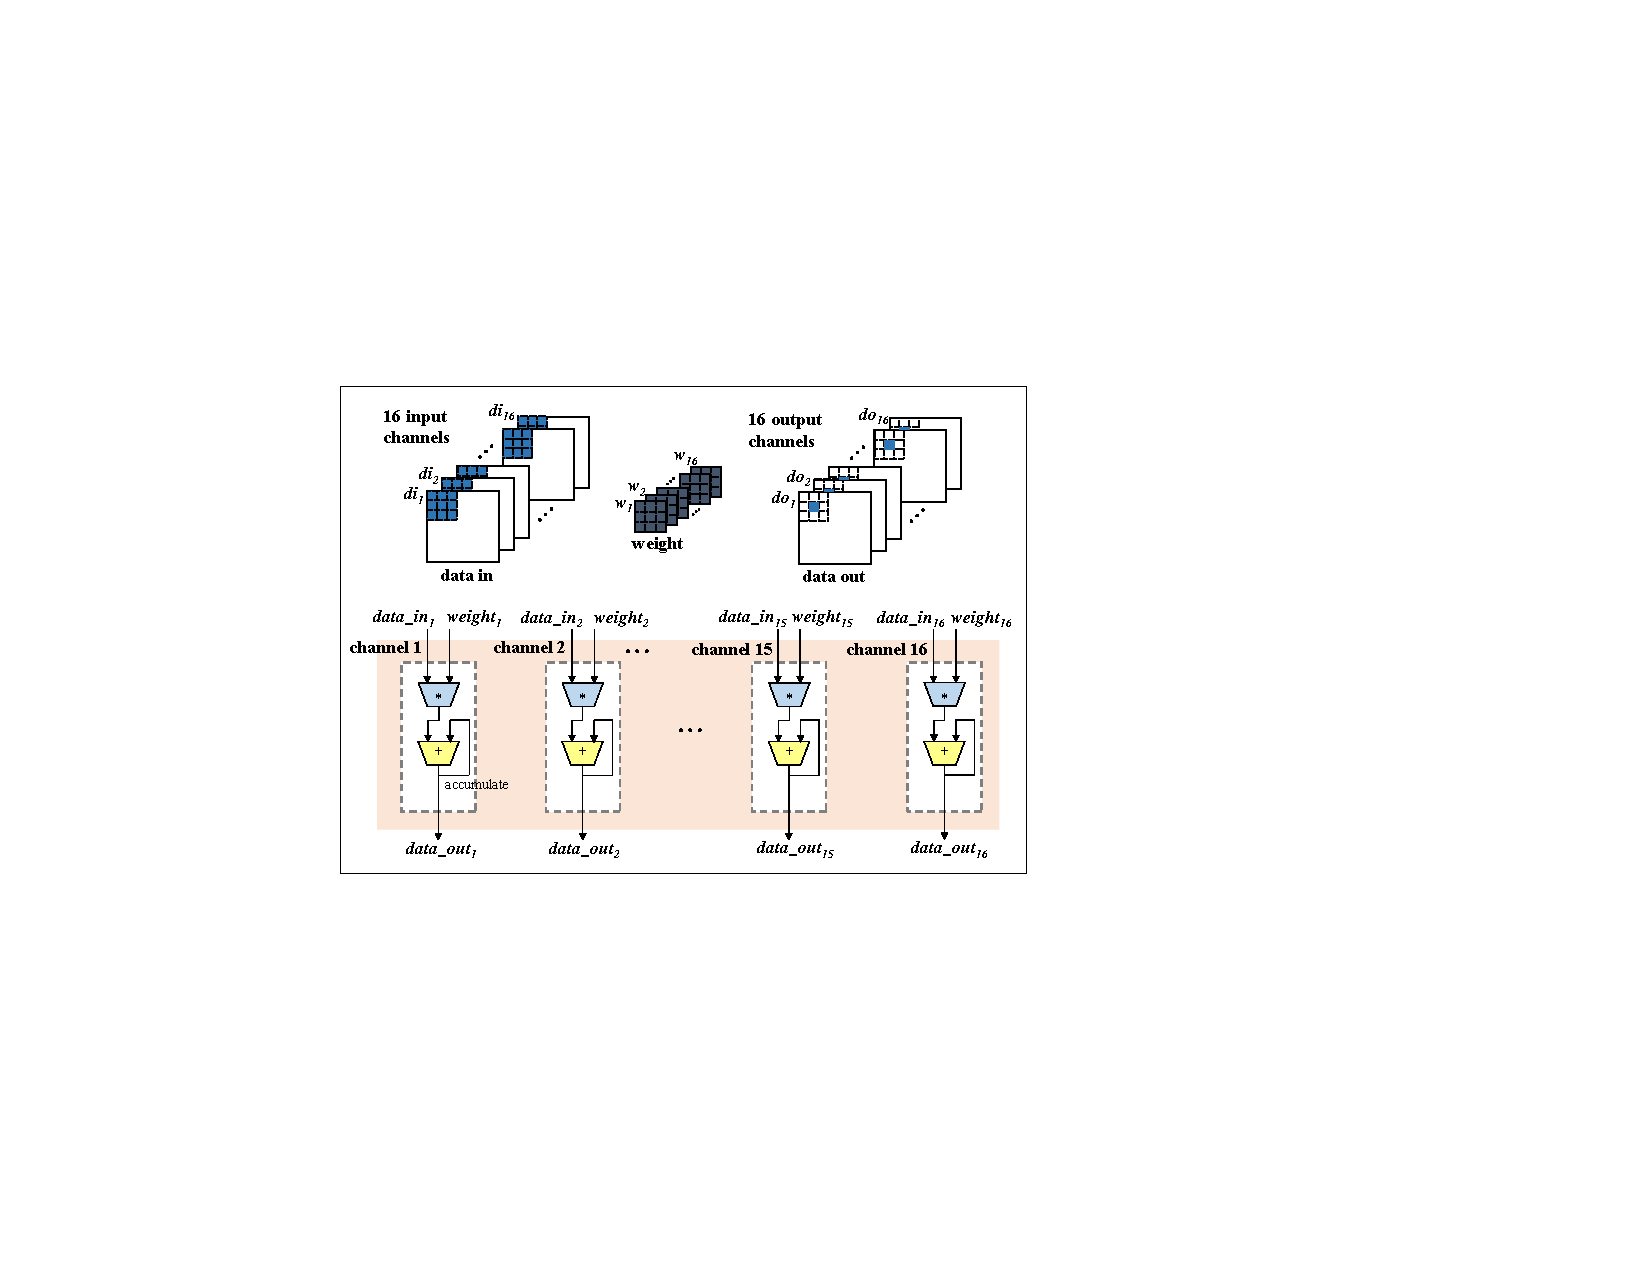
\includegraphics[width=0.7\textwidth]{dw_3x3.pdf}\\
  \vspace{-12pt}
  \caption{Depth-wise $3 \times 3$ convolutional IP design}\label{fig:3x3IP}
  \vspace{-12pt}
\end{figure}



\begin{table}[]
\centering
\caption{Performance of Depth-Wise $3 \times 3$ IP\vspace{-6pt} on Pynq-z1 Board \cite{r3}} \label{tab:dw_conv}
\renewcommand{\arraystretch}{1.1}
\setlength{\tabcolsep}{4pt}
\begin{tabular}{|c | c | c | c c c| }
\hline 
 \multirow{2}{*}{IP} & Paral. & Latency & \multicolumn{3}{c|}{Resource} \\ \cline{4-6}
 	& Factor  & \# of cycles & LUT & DSP & Flip-Flop  \\
 \hline \hline

DW-Conv & 4 & 53206 &  1866 (1.4\%) & 16 (7.3\%)& 722 (0.7\%)  \\
 3x3  	& 8 & 38807 &  2177 (1.2\%)& 16 (7.3\%) & 1549 (1.5\%) \\
 		& 16 & 18117 &  4394 (8.3\%) & 36 (16.4\%)& 2027 (2.0\%)\\ \hline
 
DW-Conv	  & 4 & 120075 &  2001 (3.8\%) & 16 (7.3\%) & 738 (0.7\%) \\
5x5		  & 8 & 64007 &  2668 (5.0\%) & 16 (7.3\%) & 554 (0.5\%)  \\
 		  & 16 & 30996 &  4966 (9.3\%) & 36 (16.4\%)& 1045 (1.0\%) \\ \hline
 		  
 \hline
\end{tabular}
\end{table}

\subsection{Point-wise Convolution $1 \times 1$ IP \label{sec:pw1x1}}

The point-wise conv $1 \times 1$ IP is usually used after a depthwise separable convolution to combine the output channels, as described in Section \ref{sec:dw_conv}.
Actually it can be regarded as a special case of a standard convolution computation, which have been discussed in Section \ref{Sec:Para_Conv}, 
so we omit detailed descriptions here.
Similar to the depthwise conv IP, Table \ref{tab:conv_1x1}
shows its performance and resource usage on the Pynq-Z1 board.


\begin{table}[]
\centering
\caption{Performance of Point-Wise $1 \times 1$ IP\vspace{-6pt}} \label{tab:conv_1x1}
\renewcommand{\arraystretch}{1.1}
\setlength{\tabcolsep}{4pt}
\begin{tabular}{|c | c | c | c c c| }
\hline 
 \multirow{2}{*}{IP} & Paral. & Latency & \multicolumn{3}{c|}{Resource} \\ \cline{4-6}
 	& Factor  & \# of clks & LUT & DSP & Flip-Flop  \\
 \hline \hline

 Conv    & 4 & 50012 &  3318 (6.2\%) & 48 (21.8\%) & 4517 (4.6\%) \\
  1x1    & 8 & 29875 &   5076 (9.5\%) & 64 (29.1\%) & 4920 (4.6\%) \\
	     & 16 & 14378 &  11871 (22.3\%) & 130 (59.1\%) & 10580 (9.9\%) \\ \hline
 
 \hline
\end{tabular}
\end{table}

\subsection{Down-sampling (pooling) IP}

\subsubsection{Introduction}

Down sampling, also called pooling, is another very common component in most deep neural networks. Pooling is used to reduce the spatial dimensions,
which helps gain computation performance, avoid over-fitting and improve translation invariance.
We omit the descriptions which are similar to depth-wise seperable IPs and only introduce the differences.

\begin{itemize}
    \item {
\textbf{Input and Output:} The inputs and outputs of pooling IP are similar to the depth-wise conv IP but no weights are required.
The input/out data shall also be stored in the on-chip memory.
    }
    \item {
\textbf{Configurable Parameters:} 
The parameters for Pooling $K \times K$ IP include:
\begin{enumerate}
    \item {
    Pooling size $K$, which indicates how much the input is down sampled by its spacial dimension. Most common choices are $K=2$ and $K=3$.
    When $K=2$, the $x$ and $y$ dimensions of the input data are downsampled by a factor of 2, and when $K=3$, $x$ and $y$ dimensions are downsampled by a factor of 3.
    }
    \item {
    Pooling method. We support three most commonly used pooling methods: max pooling, average pooling and sum pooling.
    }
    \item {
    Input feature map dimension $(H_{in}, W_{in}, C_{in})$. Similar to depthwise conv IP, the output data dimension is decided by the pooling size.
    }
    \item {
    Parallel degree $P$ along $C$ dimension, data precision of input/output feature map. These parameters are similar to depthwise conv IP.
    }
\end{enumerate}
    }
    
    \item {
    \textbf{Resource and Performance:} In Table \ref{tab:pool} we provide some performance data of pooling IP.
    The configuration is $K=2$, $S=1$, and it is demonstrated using max pooling method.
    }
    
\end{itemize}



\begin{table}[]
\centering
\caption{Performance of Max Pooling $2 \times 2$ IP\vspace{-12pt}} \label{tab:pool}
\renewcommand{\arraystretch}{1.1}
\setlength{\tabcolsep}{4pt}
\begin{tabular}{|c | c | c | c c c| }
\hline 
 \multirow{2}{*}{IP} & Paral. & Latency & \multicolumn{3}{c|}{Resource} \\ \cline{4-6}
 	& Factor  & \# of clks & LUT & DSP & Flip-Flop  \\
 \hline \hline

Pooling & 4 & 2805 &  1037 (2.0\%) & 4 (1.8\%) & 825 (0.8\%)  \\
 2x2    & 8 & 1411 &  895 (1.7\%) & 4 (1.8\%) & 758 (0.7\%)  \\
 	    & 16 & 815 &  807 (1.5\%) & 4 (1.8\%) & 739 (0.7\%)  \\ \hline
 
 \hline
\end{tabular}
\end{table}

\subsection{Bounding Box Regression}

Most IPs we provide are convolution and pooling, which are mostly used for feature extraction in image classification.
In order to support more types of deep neural networks for different applications, we provide an IP for object detection task.
Different from image classification, object detection requires the neural network to draw a bounding box on the detected object.
It is usually done by a bounding box regression component after convolutional layers. For this purpose, we borrow the regression algorithm from the popular YOLO \cite{r7}, and implement it as a configurable IP on FPGA.



The input of this IP is the feature map of the last convolution layer, and the output is the coordinates of the detected bounding boxes.
The configurable parameters of this IP include:
1) the input feature map dimension; 2) the intermediate data precision during regression; and 3) the number of anchor boxes and their aspect ratios, as described in \cite{r7}.
It provides the flexibility that the user can alter this IP according to the object features to be detected.


\subsection{Long-term Recurrent Convolution Network IP}
\subsubsection{Introduction}
Apart from General purpose DNN component IPs, we also developed a image content recognition IP based on Long-term Recurrent Convolution Network. The IP takes image as input and generates descriptive sentence as output. The  overall network flow is shown in figure \ref{fig:LRCN}. The input image is first processed by the CNN module for feature extraction. The extracted feature vector is then fed into the RNN module for recurrent word generation. The LRCN computation flow is implemented and packed into a single IP with the structure shown in figure \ref{fig:LRCN_bd}. The IP have two memory AXI interface for input/output put data transportation and one block control interface for operation control. The input interface module is responsible for reading in input data (including image data and neral network parameters) and stream the data into CNN component and LSTM component in requested order. The output interface module is responsible for writing data out back to the off chip memory.

\subsubsection{Interface}
The input and output interface between IP and DDR are memory mapped AXI4 bus protocol. The bus width is 512 bit. The Control interface are AXI-lite GPIO register interface .

\begin{figure}[h]
  \centering
  % Requires \usepackage{graphicx}
  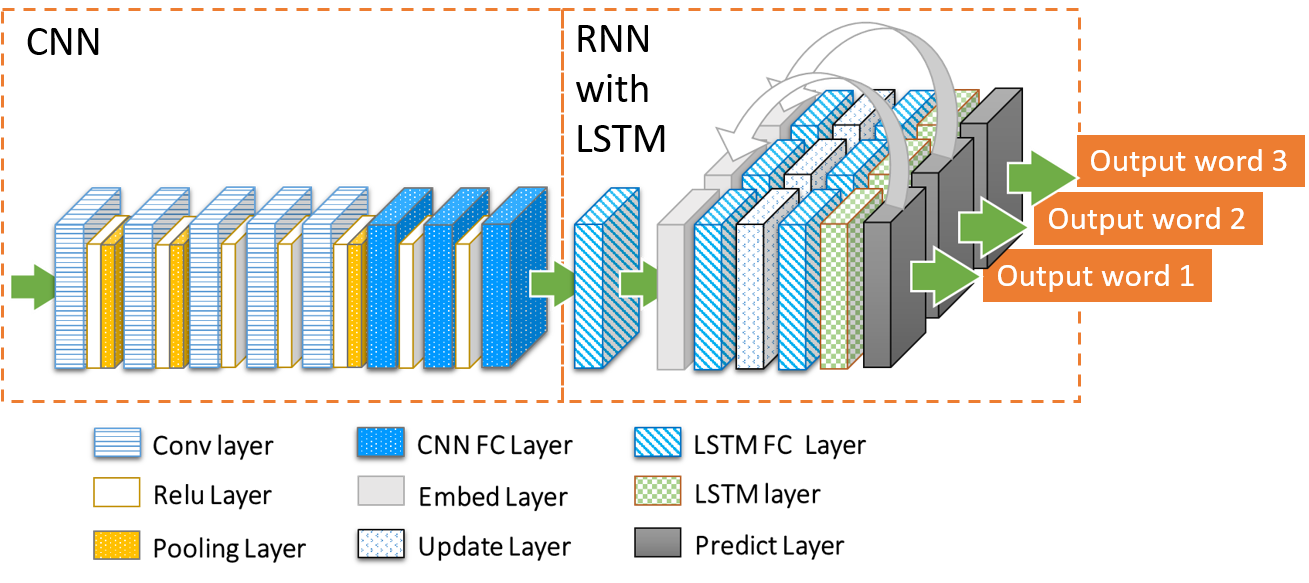
\includegraphics[width=0.7\textwidth]{LRCN.png}\\
  \vspace{-12pt}
  \caption{LRCN Network Flow}\label{fig:LRCN}
  \vspace{-12pt}
\end{figure}

\begin{figure}[h]
  \centering
  % Requires \usepackage{graphicx}
  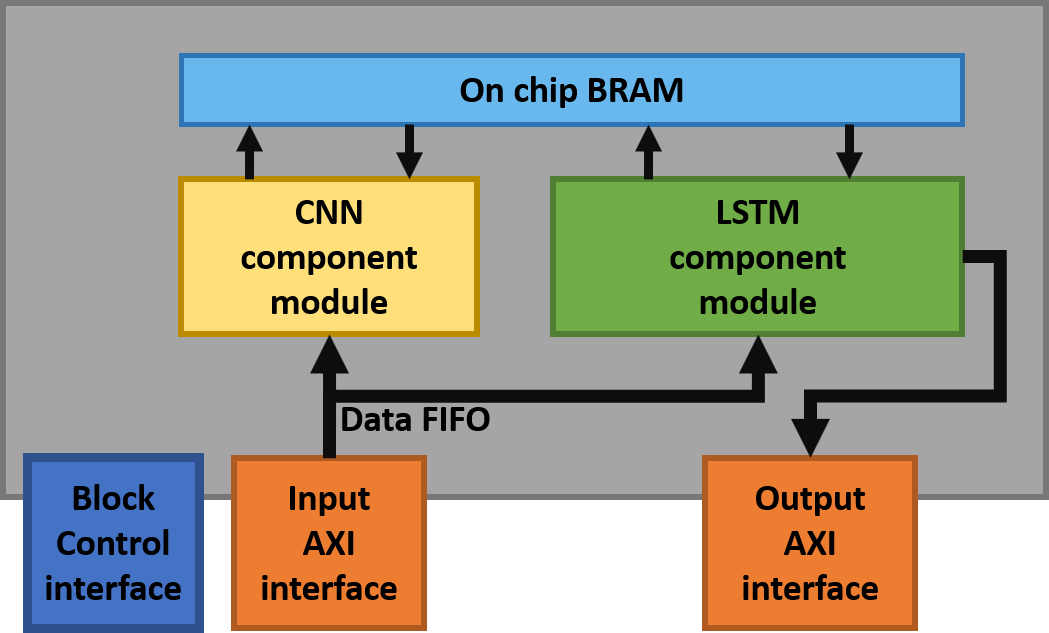
\includegraphics[width=0.7\textwidth]{lrcn_block_diagram.png}\\
  \vspace{-12pt}
  \caption{LRCN IP Structure}\label{fig:LRCN_bd}
  \vspace{-12pt}
\end{figure}

\begin{itemize}
    \item {
\textbf{Input and Output:} The IP accepts image and rearranged weight data as input and generates word index sequence as the output.
    }
    \item {
\textbf{Configurable Components:} 
The CNN component and RNN component is composed by configurable convolution and fully connected IPs. The users may alter the those IP for different CNN or LSTM structure.

\begin{enumerate}
    \item {
    Convolution Module, The convolution IP is designed to receive weight data in stream interface to achieve best performance. Configurable parameters include: input dimensions $IH \times IH\times ID$, output dimensions $OH \times OH\times OD$, kernel dimensions $FW \times FH $, data precision (8 bit, 12bit or 16 bit) and input/output parallel factor (8 or 16).
    }
    \item {
    Fully Connected Module, The convolution IP is designed to receive weight data in stream interface to achieve best performance. Configurable parameters include: input vector length $ID$, output vector length $OD$, data precision (8 bit, 12bit or 16 bit) and input/output parallel factor (8 or 16).
    }
\end{enumerate}
    }
    
\end{itemize}

\subsubsection{Resource and Performance:} 
We collect the resoruce and performance data of the image content recognition IP with AlexNet as CNN component and LSTM as the RNN component. We used Personal IP as the host machine and PCIe as the host-chip data transmission interface. The statistic is shown in Table \ref{tab:resourec_lrcn} and Table \ref{tab:perf_lrcn}

\begin{table}[h]
\centering
\caption{Resource Consumption of LRCN\vspace{-10pt}} \label{tab:resourec_lrcn}
\setlength{\tabcolsep}{4pt}
\begin{tabular}{|c | c |  c| c|}
\hline 
BRAM & DSP & Flip-Flop & LUT \\
\hline
1508 & 3130 & 321195 & 316250 \\
\hline
\end{tabular}
\end{table}

\begin{table}[h]
\centering
\caption{Performance Result of LRCN\vspace{-10pt}} \label{tab:perf_lrcn}
\setlength{\tabcolsep}{4pt}
\begin{tabular}{|c | c |  c| c|}
\hline 
Frequency & latency & Power & Efficiency \\
\hline
100Mhz & 0.04s & 23.6W & 0.94j/pic \\
\hline
\end{tabular}
\end{table}
    



\begin{thebibliography}{9}


\bibitem{r1}
L. Sifre. Rigid-motion scattering for image classification.
PhD thesis, Ph. D. thesis, 2014.

\bibitem{r2}
S. Ioffe and C. Szegedy. Batch normalization: Accelerating
deep network training by reducing internal covariate shift.
arXiv preprint arXiv:1502.03167, 2015.

\bibitem{r3}
https://reference.digilentinc.com/reference/programmable-logic/pynq-z1/start

\bibitem{r4}
Howard, Andrew G., et al. "Mobilenets: Efficient convolutional neural networks for mobile vision applications." arXiv preprint arXiv:1704.04861 (2017).

\bibitem{r5}
C. Szegedy, W. Liu, Y. Jia, P. Sermanet, S. Reed,
D. Anguelov, D. Erhan, V. Vanhoucke, and A. Rabinovich.
Going deeper with convolutions. In Proceedings of the IEEE
Conference on Computer Vision and Pattern Recognition,
pages 1–9, 2015.

\bibitem{r6}
K. Simonyan and A. Zisserman. Very deep convolutional
networks for large-scale image recognition. arXiv preprint
arXiv:1409.1556, 2014.

\bibitem{r7}
Redmon, Joseph, et al. "You only look once: Unified, real-time object detection." Proceedings of the IEEE conference on computer vision and pattern recognition. 2016.


\end{thebibliography}

\end{document}